\documentclass{article}

\usepackage[paper=letterpaper,margin=2cm]{geometry} % Set Margins

%% Math and math fonts
\usepackage{amsmath, amsthm, amssymb, amsfonts}
\usepackage{bbm} % for \mathbbm{1}

% Color
\usepackage{color, xcolor}

% Misc
\usepackage{environ}  % \collect@body in asmmath
\usepackage{graphicx} % \includegraphics options
\usepackage{mdframed} % text boxes
\usepackage{indentfirst} % Indent first paragraph after section header
\usepackage[shortlabels]{enumitem} % Control enumerate items with [(a)]
\usepackage{comment} % Comments
\usepackage{fancyhdr} % Headers and footers

% Tables
\usepackage{array}

% Sub-figures and figure placement
\usepackage{caption}
\usepackage{subcaption}
\usepackage{float} 

% Graphing
\usepackage{pgfplots}
\pgfplotsset{compat=1.17}
\usepackage{tikz}

% Title Placement
\usepackage{titling}
\setlength{\droptitle}{-6em}

% %%%% Theme %%%% % Colors from https://yaleidentity.yale.edu/web
% \definecolor{YaleBlue1}{HTML}{00356b}
% \definecolor{YaleBlue2}{HTML}{286dc0}
% \definecolor{YaleBlue3}{HTML}{63aaff}
% \definecolor{YaleGray1}{HTML}{222222}
% \definecolor{YaleGray2}{HTML}{4a4a4a}
% \definecolor{YaleGray3}{HTML}{978d85}
% \definecolor{YaleGray4}{HTML}{dddddd}
% \definecolor{YaleWhite}{HTML}{f9f9f9}
% \definecolor{YaleGreen}{HTML}{5f712d}
% \definecolor{YaleOrange}{HTML}{bd5319}

%set indent to 
\setlength{\parindent}{0pt}

%for headers 
\pagestyle{fancy}
\fancyhf{} % for header/footer

\lhead{Creel}
\rhead{Fisheries}

\title{Week Seven -- More Optimal Allocation but Fisheries Now}
\author{Andie Creel}
\date{March 1st, 2023}

% Hyper refs
\usepackage{hyperref}
\hypersetup{
    colorlinks=true,
    linkcolor=blue,
    urlcolor  = blue,
    filecolor=magenta,      
    urlcolor=blue,
    citecolor = blue,
    anchorcolor = blue
}

% Citation management
\usepackage{natbib}
\bibliographystyle{abbrvnat}
\setcitestyle{authordate,open={(},close={)}}

\begin{document}
\maketitle

\section{Fisheries}
\textbf{Continuous Schaefer Harvest Function}
\begin{align}
    h = q E S
    \label{schaefer}
\end{align}
where $q$ is a parameter measuring catch-ability (fraction of population you catch for one unit of effort) , $E$ is effort, and $S$ is stock. The catch-ability could change with an exogenous shock.\footnote{Exogenous is economists' fancy word for random. You can think of this as an unpredictable shock.} \\

\textbf{Discrete Schaefer Harvest Function}:
\begin{align}
    h = S(1 - e^{-qe})
\end{align}

\textbf{Costs of harvest}
\begin{align}
    c_h > 0
\end{align}
\textit{i.e.,} the first derivative of costs with respect to (wrt) harvest positive, meaning cost is increasing as harvest increases.

\begin{align}
    c_{hh} >0
\end{align}
\textit{i.e.,} the second derivative of costs wrt harvest is positive, mean the cost is increasing as an increasing rate as harvest increases. Cost is a convex function wrt harvest. \\

\textbf{Dividents / Profit}
\begin{align}
    \pi &= ph - c(h) \label{divid_1} \\
    &= pqES - c(qES) \label{divid_2} 
\end{align}
where I've plugged in the schaefer harvest equation \ref{schaefer} to \ref{divid_1} to get \ref{divid_2}.\\

In a competitive equilibrium, profits will be driven to zero, $E^\infty$. This is the open access outcome. However, if we want to maximize economic yield, we would find a very different outcome. The graph of revenue on effort (figure \ref{max_econ_yeild}) shows the open access amount of effort and the maximum economic yield. \\

\begin{figure}[htp]
    \centering
    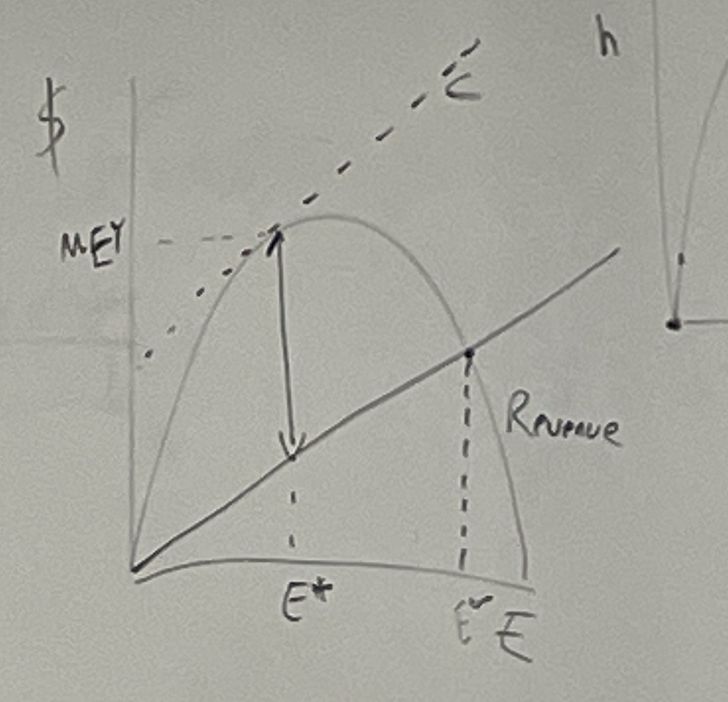
\includegraphics[width=8cm]{Screen Shot 2023-03-01 at 9.38.11 AM.png}
    \caption{}
    \label{max_econ_yeild}
\end{figure}

\subsection{Static solution for Maximum Economic Yield}
Consider a fisherman who wants to maximize his profits which is equation \ref{divid_1},

$$\pi \&= ph - c(h).$$

If he wants to maximize profit (statically) he could take the first derivative of \ref{divid_1}, set it equal to 0 and solve for the $h$ that maximizes economic yield. 

\begin{align}
    \frac{\partial \pi}{\partial h} = p - \frac{\partial c}{\partial h} = 0 \label{static}
\end{align}

The fisherman can solve \ref{static} for $h$ to maximize his profit in one time period. \\

However, this static solution does not account for how the stock is changing ($\dot s$) or the initial population. Individual fishers can't affect the behavior of the stock (their impact is so small) so their discount rate is $\delta = \infty$ because they're putting absolutely zero weight on the value of the next time period. This causes their shadow price for stock to be zero (not valuing the future behaves the same a not valuing the stock). Their individual dividend equation doesn't put any shadow price on the population of fish. However, a social planner would account for fish having a positive shadow price, so we need to use a Hamiltonian to account for dynamics through time. 

\subsection{Dynamic Solution for Max. Econ. Yield}
The social planner would place a positive value on fish in the future, so they would use a current value Hamiltonian in order to account for capital gains,
\begin{align}
    H = ph - c(s,h) + \lambda (G(s) - h)
\end{align}
where 
\begin{align}
    G(s) = rs(1 - \frac{s}{K})
\end{align}
and recall that 
\begin{align}
    capital\ gains = \lambda (G(s) - h).
\end{align}
The major difference between the Hamiltonian and the static solution is \textbf{capital gains}. Capital gains are what cause us to consider of fish may have value in the next time period. \\

To find the social planner's optimal effort, take optimality conditions. \\

Optimality Conditions: 
\begin{align}
    \frac{\partial H}{\partial h} &= p - \frac{\partial C}{\partial h} - \lambda = 0 \label{FOC_1} \\
    \frac{\partial H}{\partial s} &= \delta \lambda - \dot \lambda \label{FOC_2}
\end{align}
where \ref{FOC_1} is our first optimality condition of a Hamiltonian and \ref{FOC_2} is our second optimality condition of a Hamiltonian (Refer to section Four Lagragian vs Hamltonian notes). \\

\textbf{Finding optimal $h^*$:} If we solve \ref{FOC_1} for $h$, we'll find the socially optimal harvest level. However, it will  be a function of $\lambda$. \\

\textbf{Finding $\lambda$:} We can rearrange \ref{FOC_2} to solve for $\lambda$ which is our Euler equation (refer to week four, natural capital class notes) 
\begin{align}
    \lambda = \frac{\pi_s + \dot \lambda}{\delta - G_s(s)}
\end{align}

and then we can solve for $h^*$!\\

\textbf{Policy intervention}: To get fishermen to harvest the socially optimal level of fish $h^*$, we can set a TAX in order to get them to fish less $\tau = \lambda$. \\

\textbf{Returning for fishermen's static problem}: Now, when the fishermen solve their static problem, their costs has to take account of the tax. Their profit equation (previously \ref{divid_1}) is now 
\begin{align}
    \pi = ph - c(h) - \tau h
\end{align}
and so when the fishermen gets his own static FOC it is
\begin{align}
    \frac{\partial \pi}{\partial h} = p - \frac{\partial c}{\partial h}- \tau = 0 \label{FOC_static_tax}
\end{align}
and notice that \ref{FOC_static_tax} is the same as \ref{FOC_1} (because we choose the tax to equal to shadow price $\tau = \lambda$)!! And so our static problem's solution for the optimal $h$ will now be the same as the dynamic problems. 

\subsection{The major point}
If a fisherman doesn't benefit from owning capital (fisheries are open access), then fishermen won't consider the capital gains of having stock in the next time period (because they don't own the stock). A tax is a way to get the fisherman to harvest in the socially optimal way because it causes the fisherman's optimization problem (maximizing his dividends/profit) to mimic the social planners optimization problem (maximize dividends/profit AND capital gains). 

\section{Cap and Trade -- individual traded quotas}
Individual traded quotas (ITQs) are another way to cause fishermen to harvest at the socially optimal harvest level. ITQs are a version of cap and trade. Cap ad trade, when the cap is set correctly, will lead to the same outcome as a tax (ex. Section 1.2). 

\begin{align}
    \pi = ph - c(s,h) - y*(h - q_0)
\end{align}
Rewrite in terms of quota
\begin{align}
    \pi = ph - c(s,q) - y*(q - q_0)
\end{align}


FOC: 
\begin{align}
    \frac{\partial \pi}{\partial q} = p - \frac{\partial c}{\partial q} - y = 0
\end{align}

which mirrors \ref{FOC_static_tax} and \ref{FOC_1}. 

\end{document}